%!TEX root = ../RASD/main.tex

\subsection{User Interface} % (fold)
In this section are shown the first mock-ups of the applications of the \emph{system-to-be}.

\subsubsection{\nameref{app:mobileuser} }
\begin{figure*}[h!t]
    \centering
    \begin{subfigure}[h!t]{0.25\paperwidth}
            \includegraphics[width=\textwidth]{mockups/user-app/Register}
            \caption{Register}
    \end{subfigure}
    \hspace{0.05\paperwidth}
    \begin{subfigure}[h!t]{0.25\paperwidth}
            \includegraphics[width=\textwidth]{mockups/user-app/LogIn}
            \caption{Log In}
    \end{subfigure}
\end{figure*}
\vfill
\clearpage

\newpage
\vfill
\begin{figure*}[h!t]
    \centering
    \begin{subfigure}[h!t]{0.25\paperwidth}
            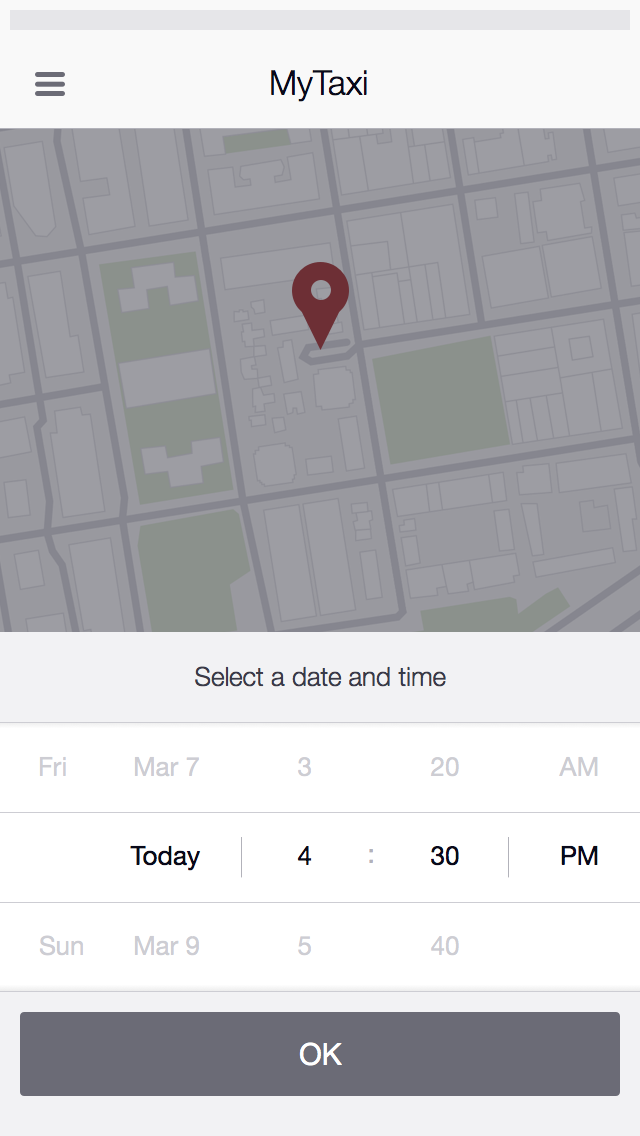
\includegraphics[width=\textwidth]{mockups/user-app/Book}
            \caption{Book}
    \end{subfigure}
    \hspace{0.05\paperwidth}
    \begin{subfigure}[h!t]{0.25\paperwidth}
            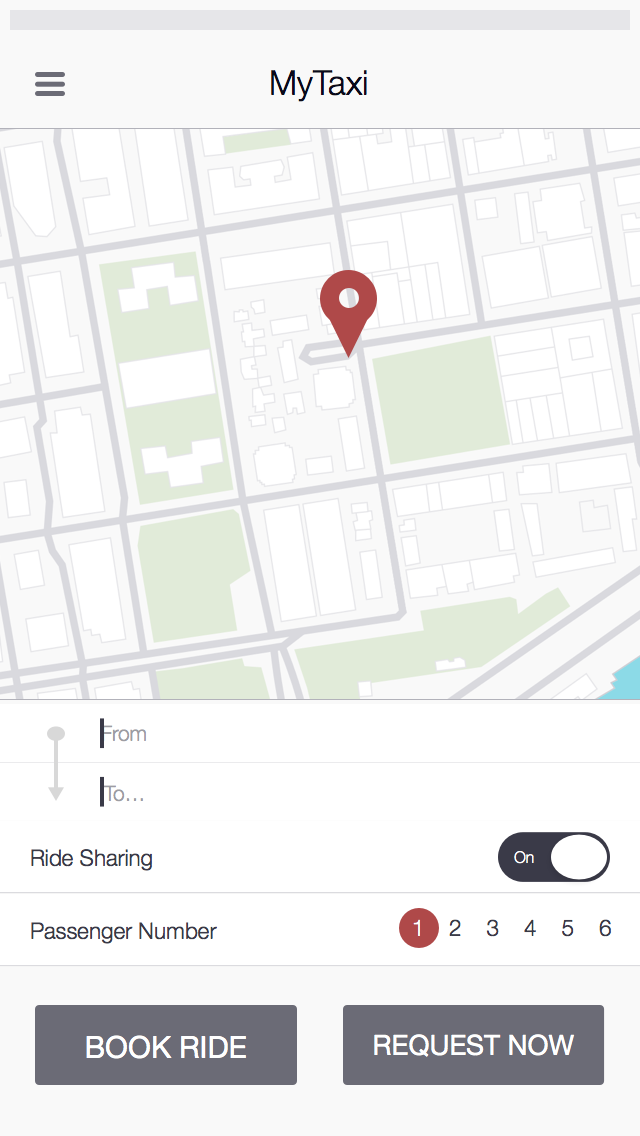
\includegraphics[width=\textwidth]{mockups/user-app/CallTaxi}
            \caption{Call}
    \end{subfigure}
\end{figure*}
\vfill
\clearpage

\newpage
\vfill
\begin{figure*}[h!t]
    \centering
    \begin{subfigure}[h!t]{0.25\paperwidth}
            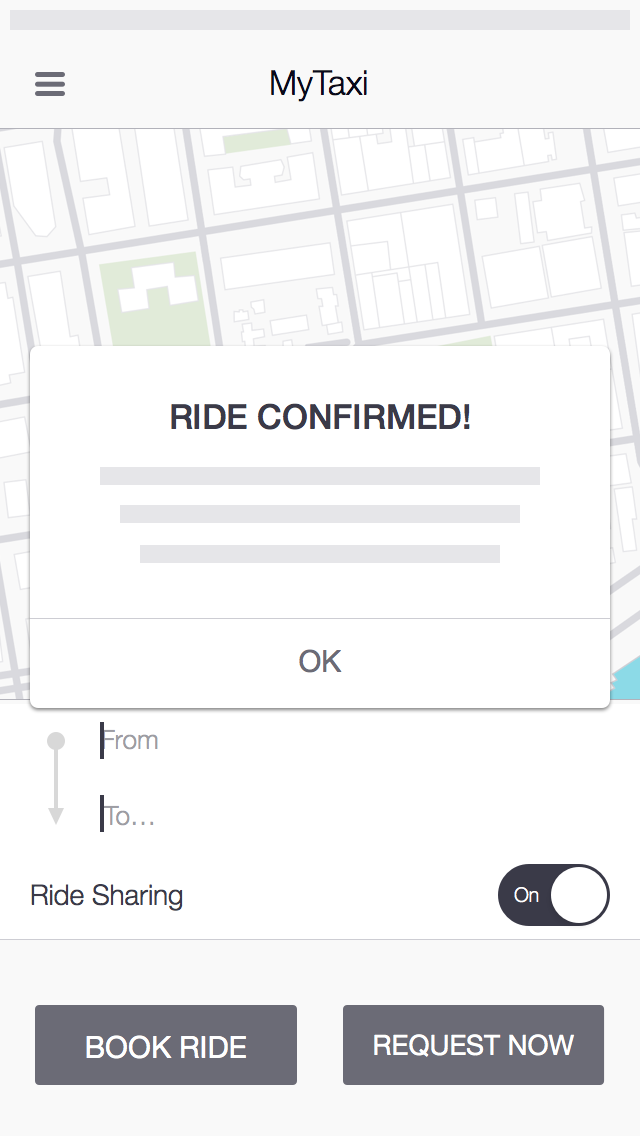
\includegraphics[width=\textwidth]{mockups/user-app/Confirm}
            \caption{Confirm}
    \end{subfigure}
    \hspace{0.05\paperwidth}
    \begin{subfigure}[h!t]{0.25\paperwidth}
            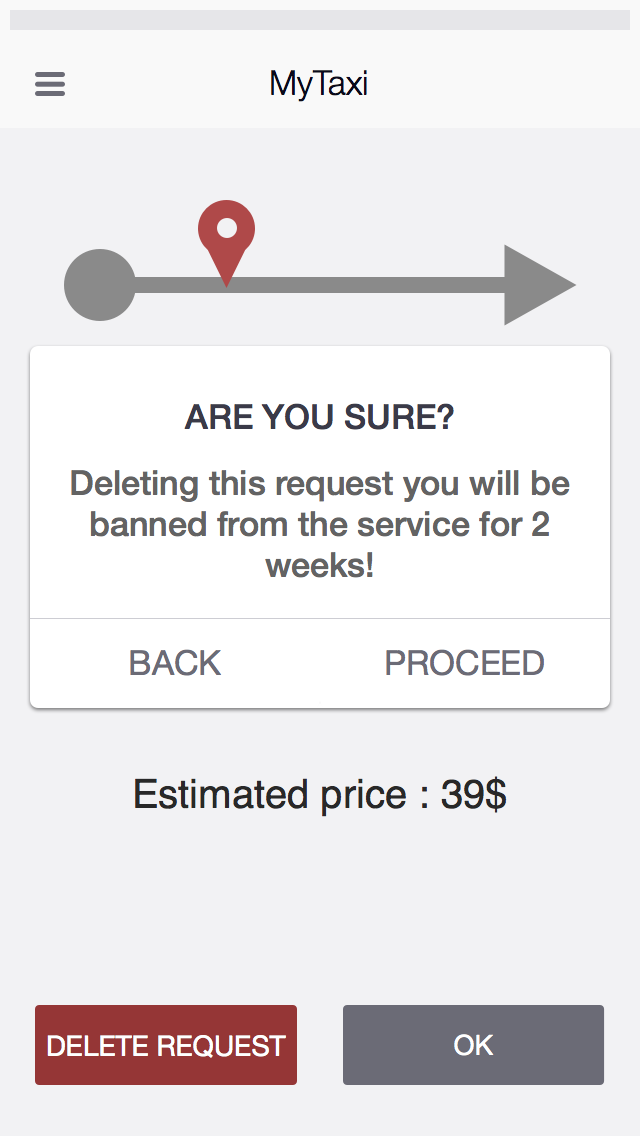
\includegraphics[width=\textwidth]{mockups/user-app/Delete}
            \caption{Delete}
    \end{subfigure}

    \begin{subfigure}[h!t]{0.25\paperwidth}
            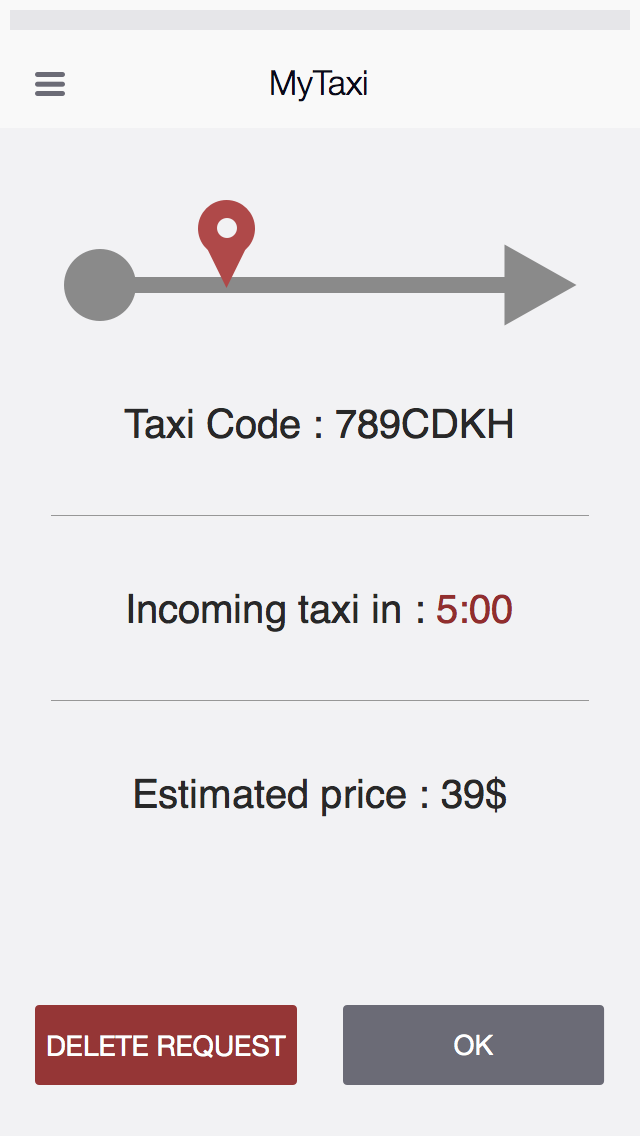
\includegraphics[width=\textwidth]{mockups/user-app/Pending}
            \caption{Pending}
    \end{subfigure}

\end{figure*}
\vfill
\clearpage


\newpage
\subsubsection{\nameref{app:web} }
\vfill
\begin{figure}[h!t]
\caption{Register}
\includegraphics[width=\textwidth]{mockups/web-app/Register}
\centering
\end{figure}
\vfill
\clearpage

\newpage
\vfill
\begin{figure}[h!t]
\caption{Login}
\includegraphics[width=\textwidth]{mockups/web-app/LogIn}
\centering
\end{figure}
\vfill
\clearpage

\newpage
\vfill
\begin{figure}[h!t]
\caption{Book}
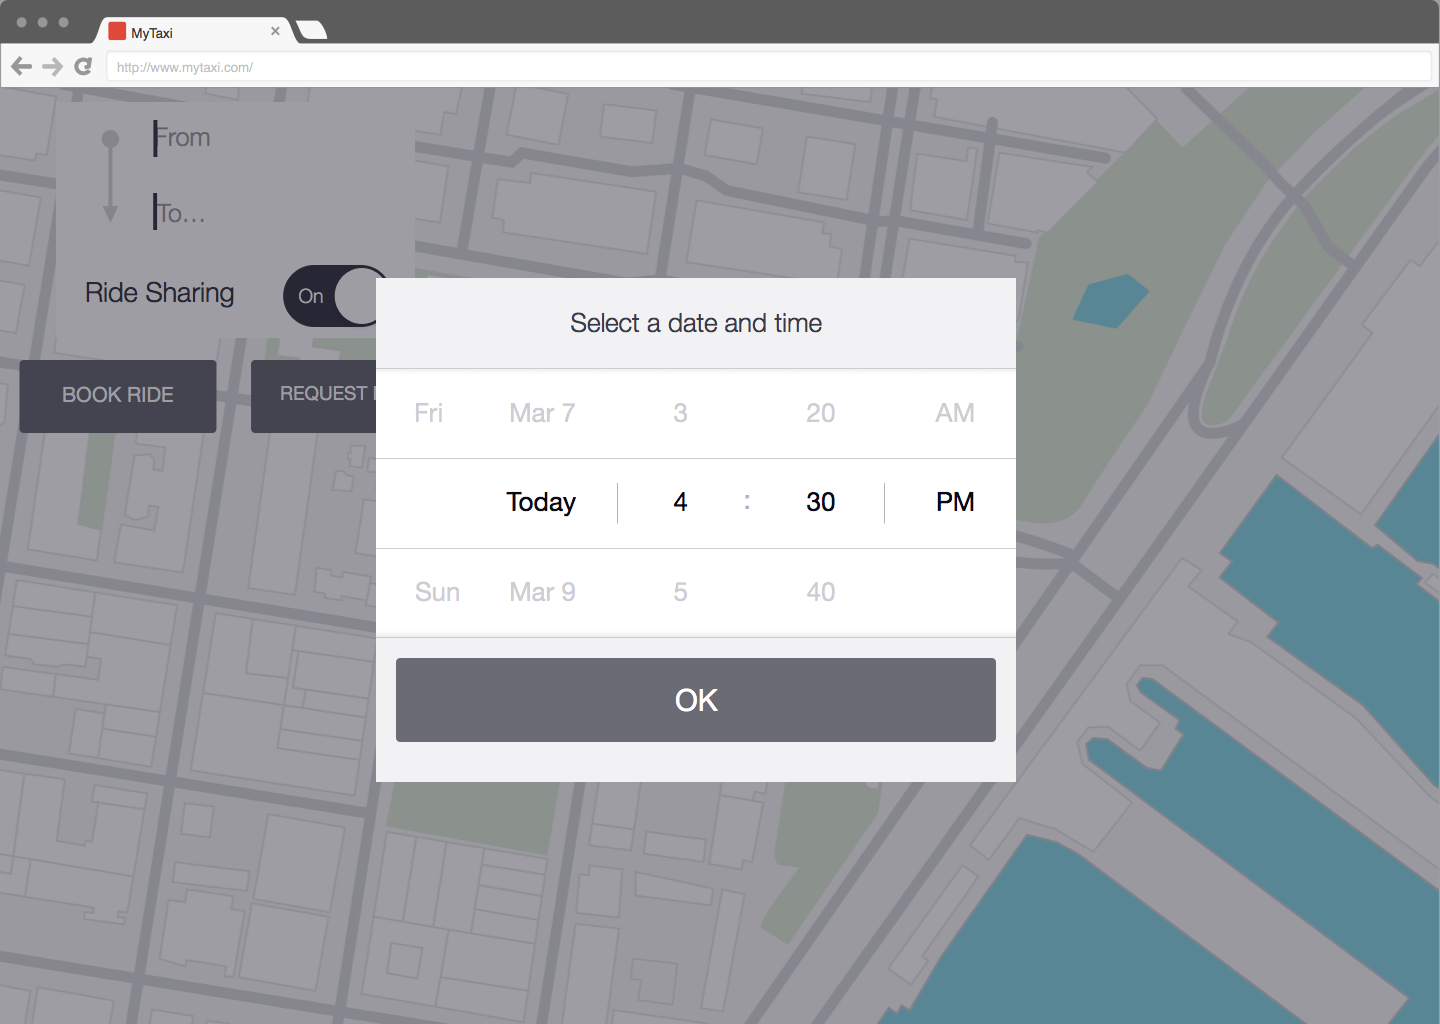
\includegraphics[width=\textwidth]{mockups/web-app/BookTaxi}
\centering
\end{figure}
\vfill
\clearpage

\newpage
\vfill
\begin{figure}[h!t]
\caption{Request}
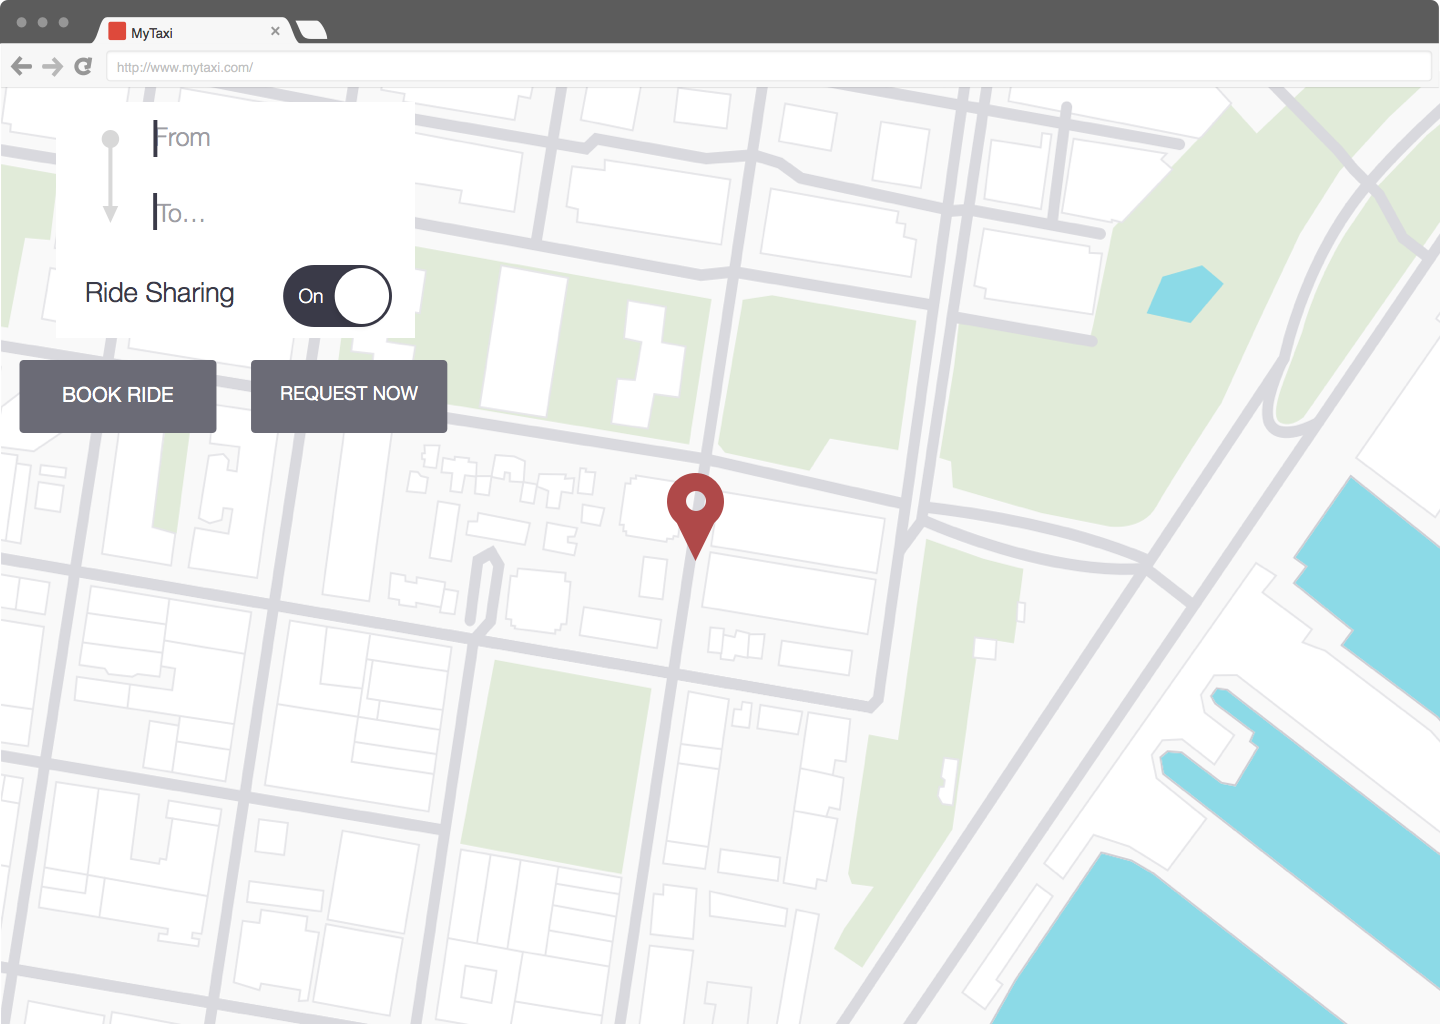
\includegraphics[width=\textwidth]{mockups/web-app/RequestTaxi}
\centering
\end{figure}
\vfill
\clearpage

\newpage
\subsubsection{\nameref{app:mobiledriver} }
\vfill
\begin{figure*}[h!t]
    \centering
    \begin{subfigure}[h!t]{0.24\paperwidth}
            \includegraphics[width=\textwidth]{mockups/driver-app/LogIn}
            \caption{Log in}
    \end{subfigure}
    \hspace{0.02\paperwidth}
    \begin{subfigure}[h!t]{0.24\paperwidth}
            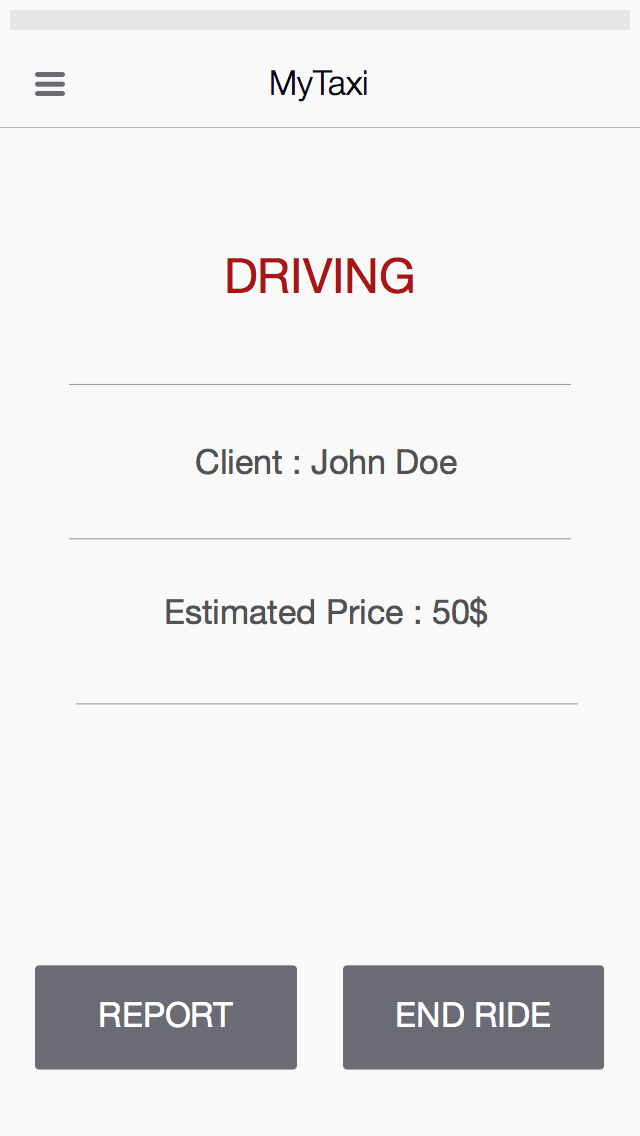
\includegraphics[width=\textwidth]{mockups/driver-app/OnRide}
            \caption{On Ride}
    \end{subfigure}
    \hspace{0.02\paperwidth}
    \begin{subfigure}[h!t]{0.24\paperwidth}
            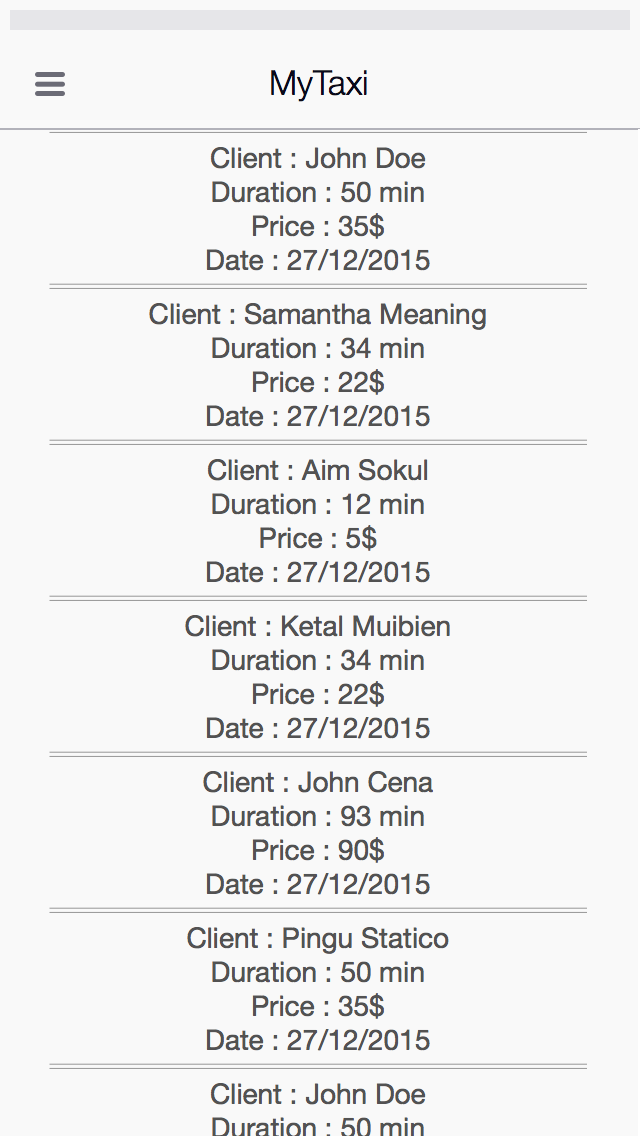
\includegraphics[width=\textwidth]{mockups/driver-app/RideHistory}
            \caption{Ride History}
    \end{subfigure}
\end{figure*}
\vfill
\clearpage


\newpage
\vfill
\begin{figure*}[h!t]
    \centering
    \begin{subfigure}[h!t]{0.25\paperwidth}
            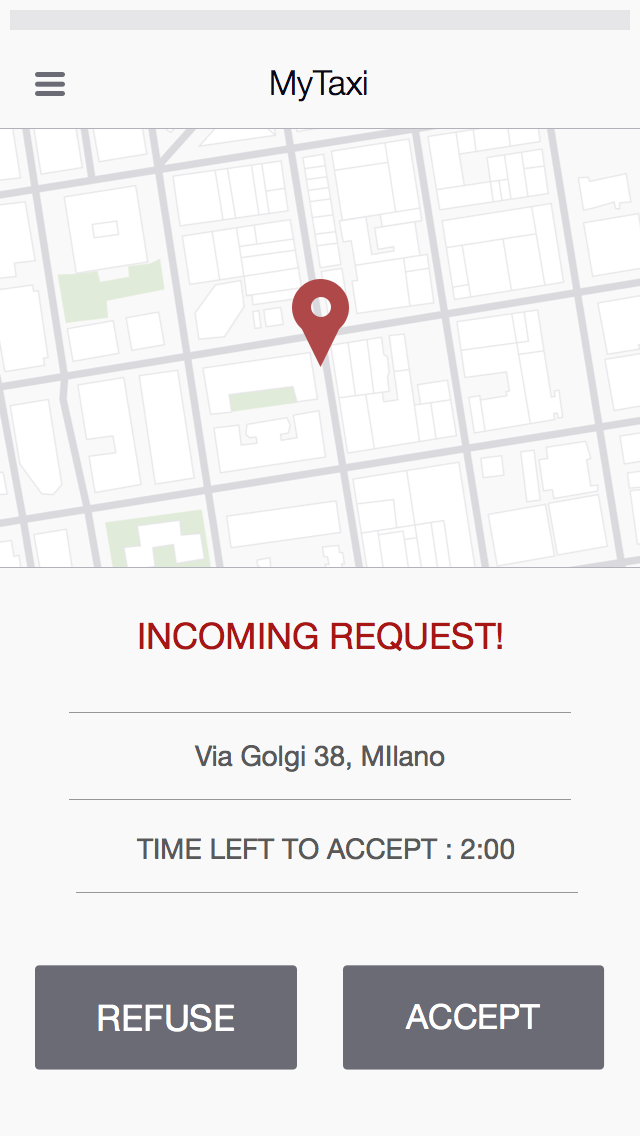
\includegraphics[width=\textwidth]{mockups/driver-app/IncomingRequest}
            \caption{Incoming Request}
    \end{subfigure}
    \hspace{0.05\paperwidth}
    \begin{subfigure}[h!t]{0.25\paperwidth}
            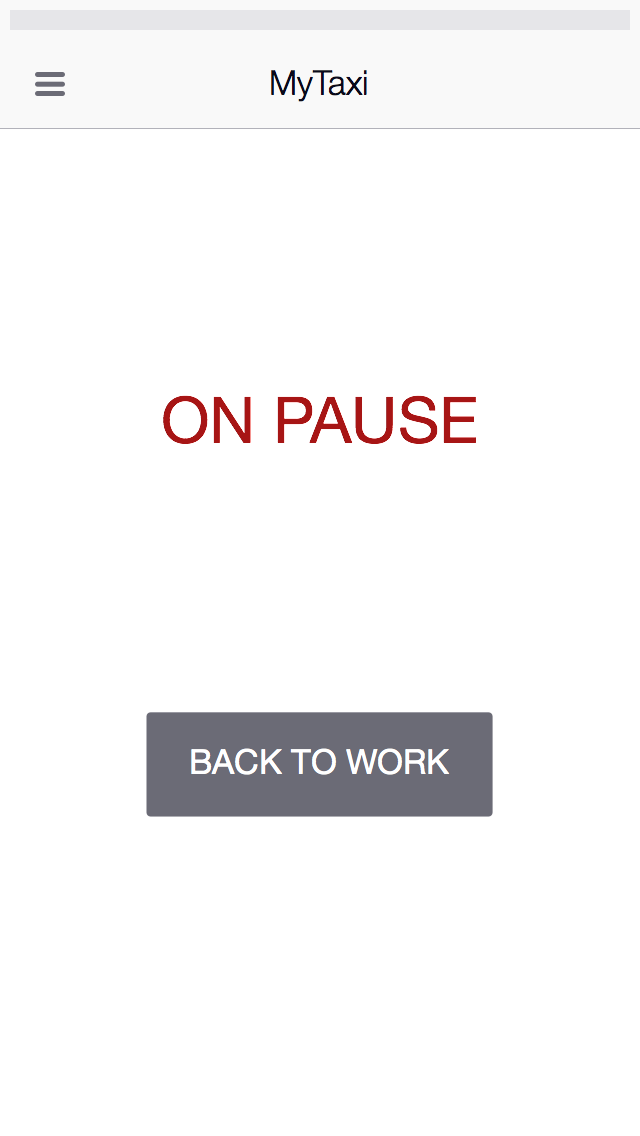
\includegraphics[width=\textwidth]{mockups/driver-app/IdleStateScreen}
            \caption{Idle State}
    \end{subfigure}
    \vspace{0.05\paperwidth}

    \begin{subfigure}[h!t]{0.25\paperwidth}
            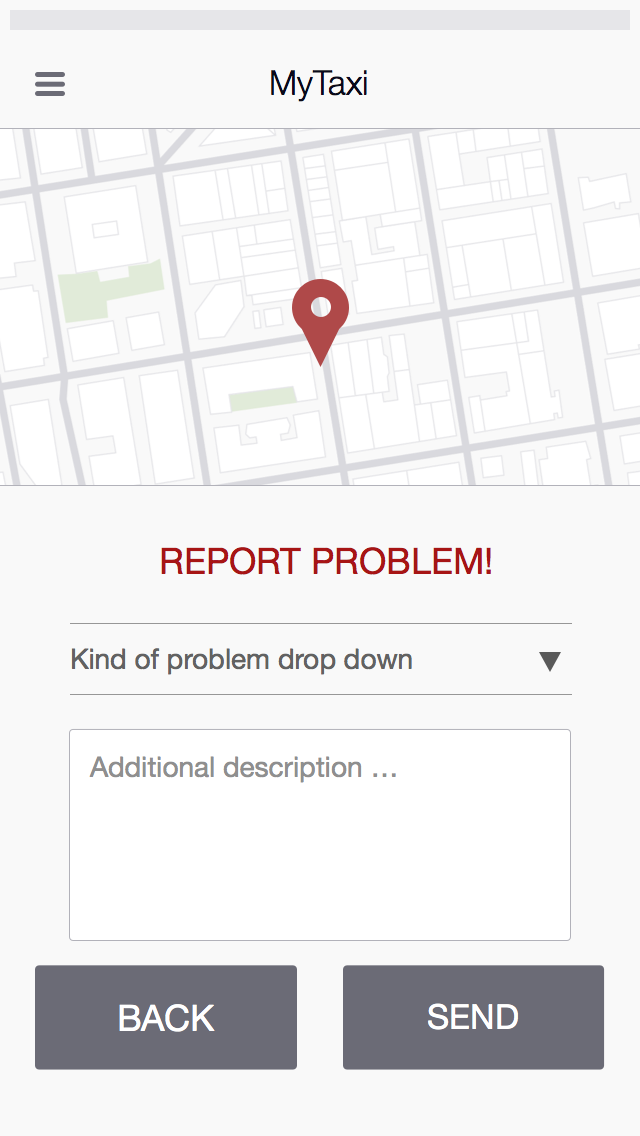
\includegraphics[width=\textwidth]{mockups/driver-app/ReportProblem}
            \caption{Report Problem}
    \end{subfigure}

\end{figure*}
\vfill
\clearpage


